\subsection{Initialization of application}
%---------------------------
%include sequence diagram for initialization here
%---------------------------

\subsection{example action: select export format}
This sequence diagram states as example for a simple action handler.
In this action the user wants the currently displayed output translated into a specified format. The sequence diagram starts when the user selects the export format in the UI. 
The SelectExportFormat poses as action handler for the selected UI element. Thus when this element is clicked, the actions run() method is called. All invoked instances are already existing, none is being created in this scenario.
The actions run() method generates the dedicated representation by requesting the currently displayed lambda terms from the ExecutionEngine instance and generating their representation.
The representation is then written into the export window that will be displayed to the user. Writing before showing this export window ensures, that at no point in time an empty window is displayed.
However, before actually displaying it, a blocker that prevents the user from interacting with any UI element, other than the export window, is enabled.

\begin{figure}[H]
	\centering
	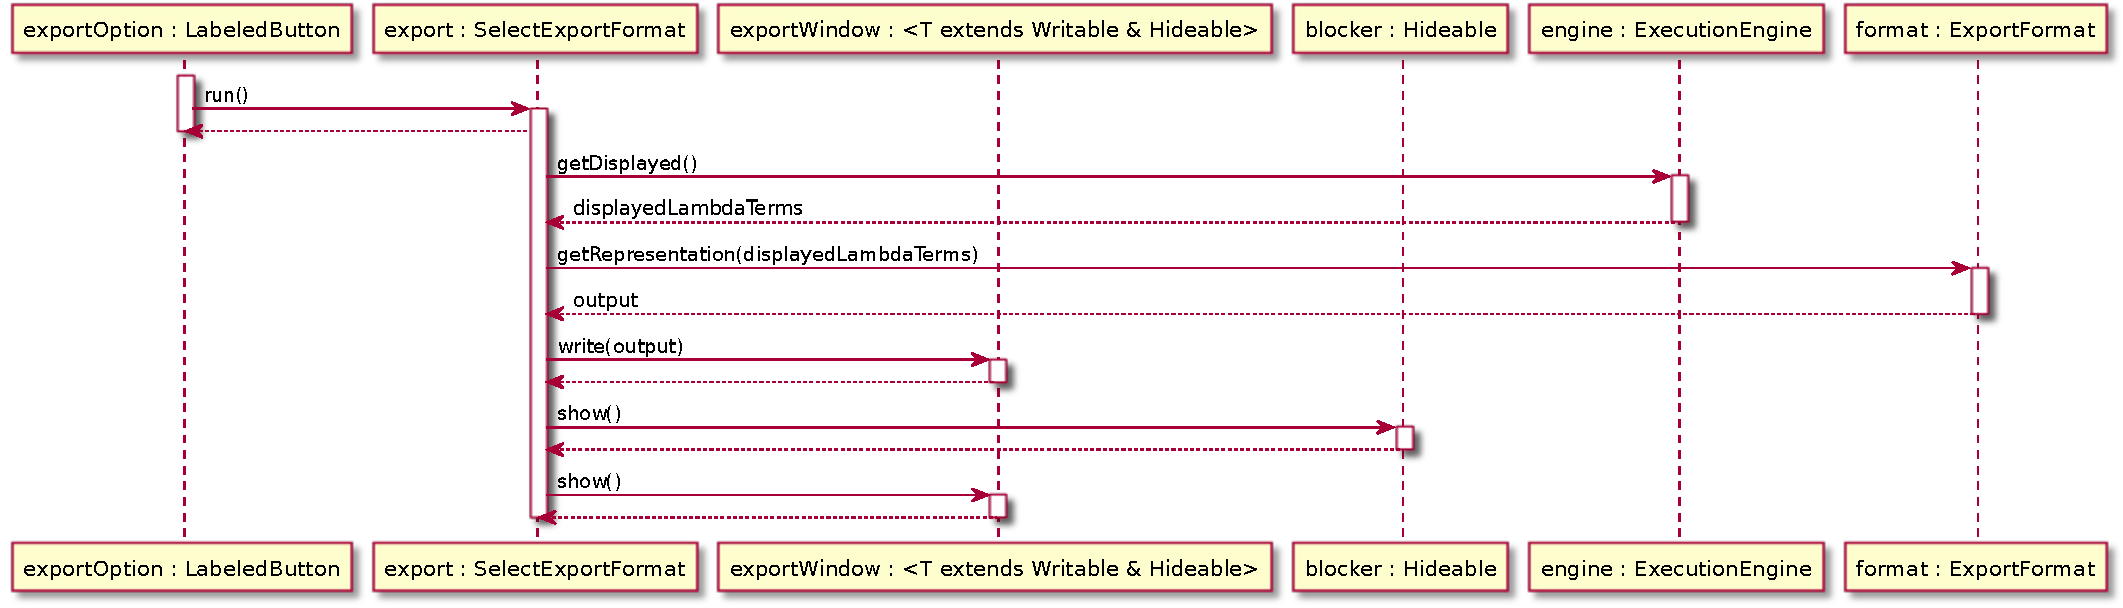
\includegraphics[width=\textwidth]{sequenceDiagrams/exportOutput}
\end{figure}

\subsection{example action: start reduction process}
%---------------------------
%include sequence diagram for action here
%---------------------------

\subsection{Beta reduction}
%---------------------------
%include text here
%---------------------------

\begin{figure}[H]
	\centering
	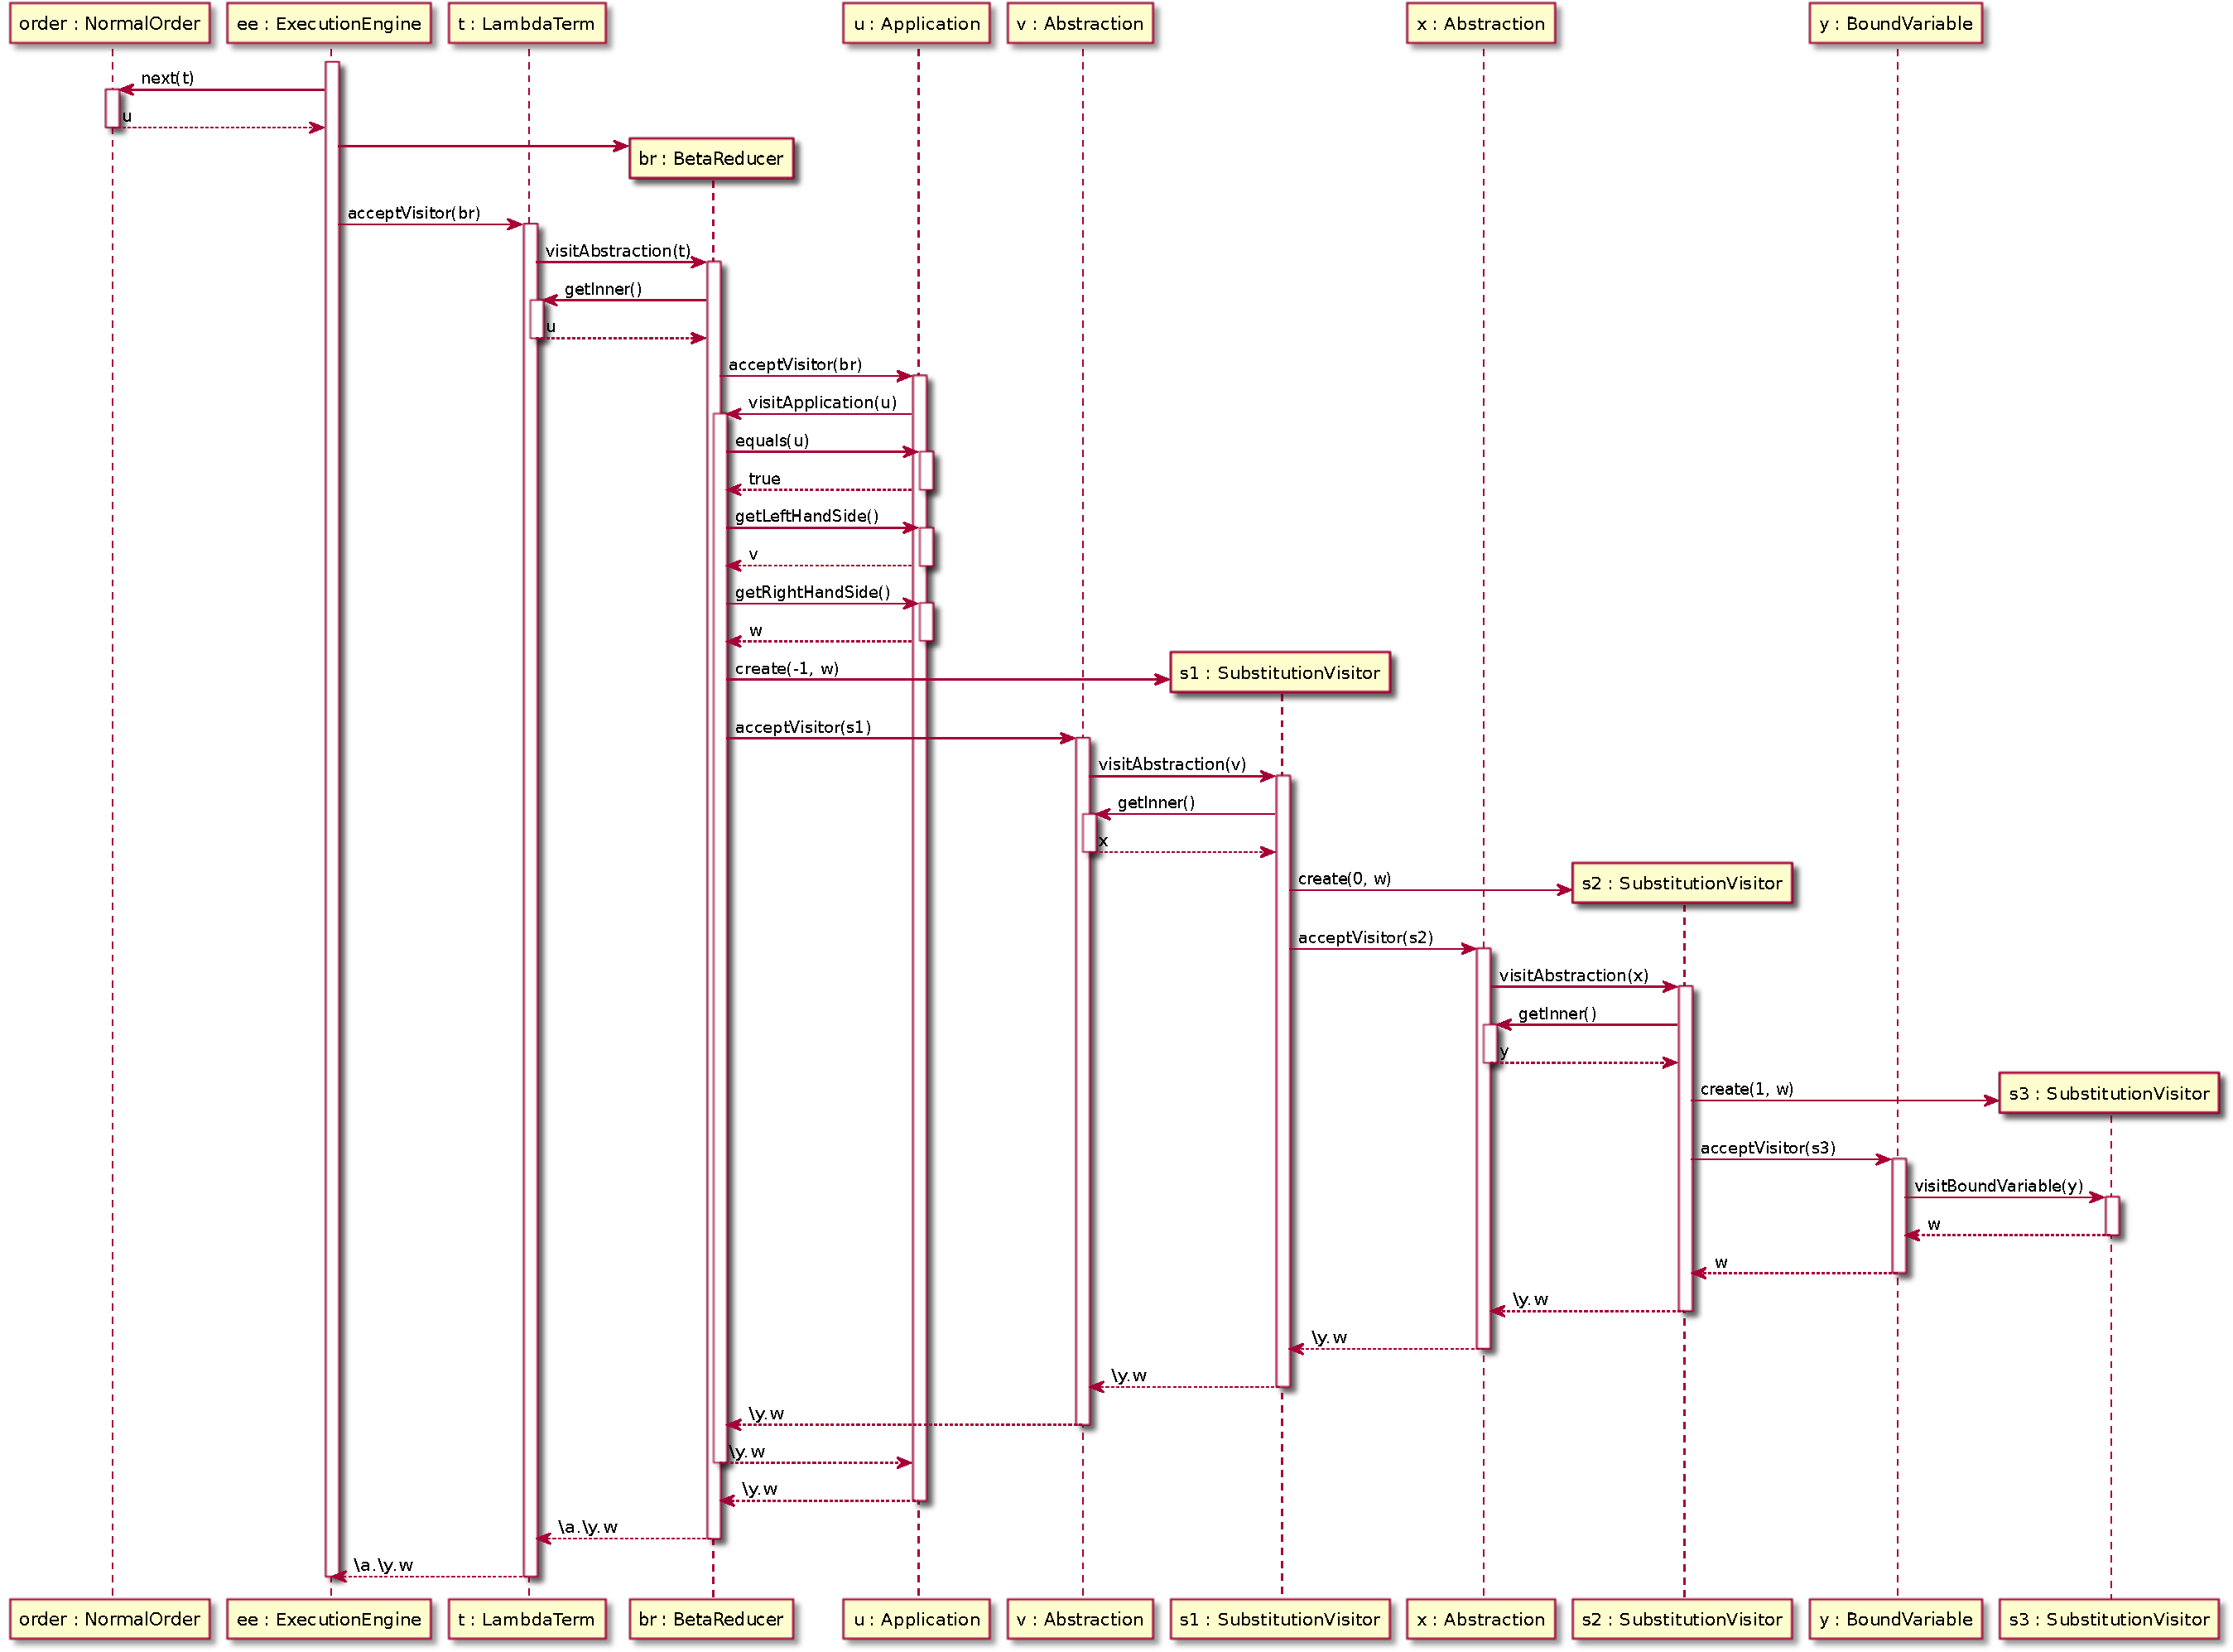
\includegraphics[width=\textwidth]{sequenceDiagrams/betaReduction}
\end{figure}

\subsection{Next term}
%---------------------------
%include text here
%---------------------------

\begin{figure}[H]
	\centering
	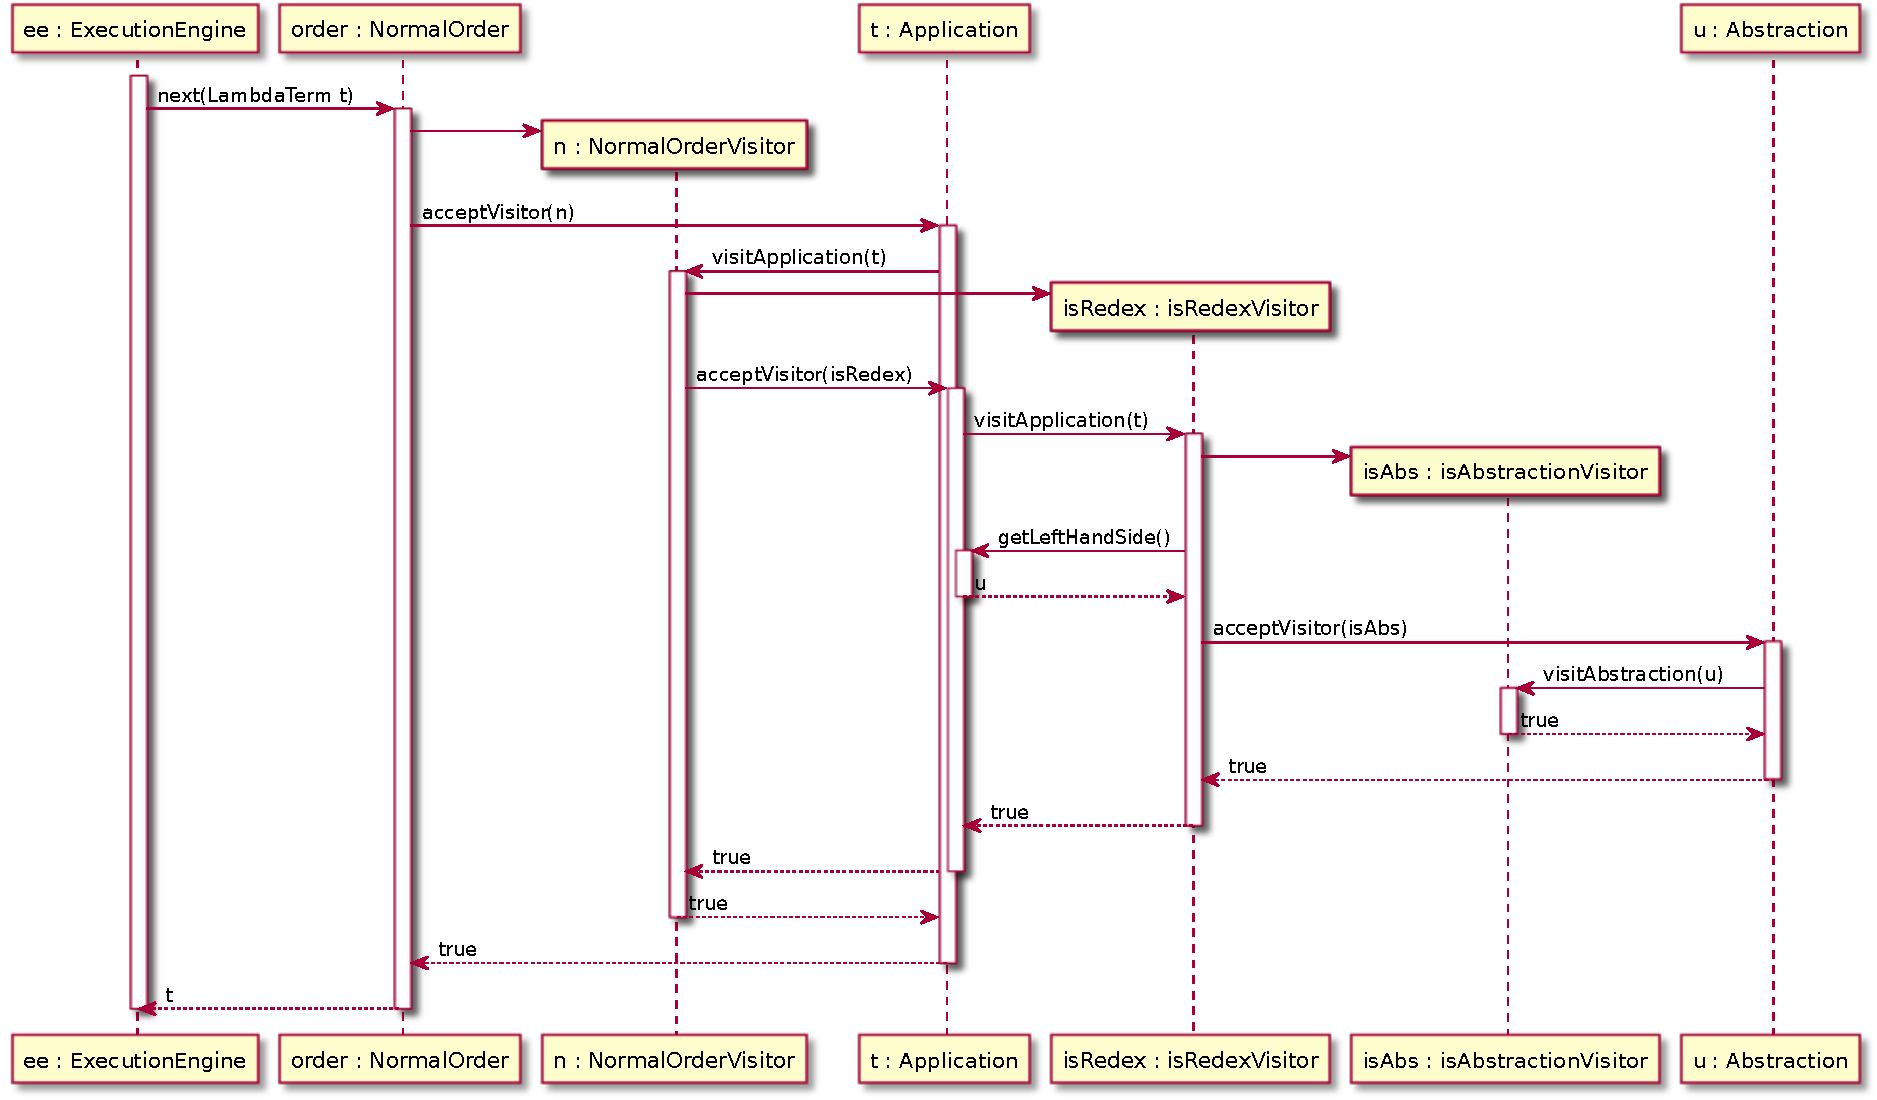
\includegraphics[width=\textwidth]{sequenceDiagrams/nextTerm}
\end{figure}

